\subsection{Virtual Ports}

\subsubsection{Introduction}
Virtual ports in the Gpio module allow for the abstraction of physical pins, enabling flexible control without altering the underlying hardware behavior. A virtual port can be mapped to a physical pin, and its behavior will correspond to the mode (input or output) of the pin it is mapped to.

This section details how virtual ports should behave when mapped to physical pins, how data flows between them, and how enable signals are managed.

\subsubsection{Physical Pin Configured as Output}
When the physical pin is configured as an output, the virtual port should mirror this configuration.

\begin{itemize}[noitemsep]
    \item \textbf{Data Flow}: The virtual port writes data to the corresponding physical pin.
    \begin{itemize}[noitemsep]
        \item Writing to the virtual port sets the output value of the physical pin.
        \item The virtual port is implicitly in output mode.
    \end{itemize}
    \item \textbf{Enable Behavior}: Writing to the virtual port acts as if writing directly to the physical pin.
    \begin{itemize}[noitemsep]
        \item Virtual port output is enabled when the physical pin output is enabled.
    \end{itemize}
\end{itemize}

\textbf{Example}:
\begin{itemize}[noitemsep]
    \item Physical pin $p$ is set as output.
    \item Virtual port $v$ is mapped to pin $p$.
    \item Writing a $1$ to virtual port $v$ sets the output of pin $p$ to $1$.
    % insert the image of the virtual ports diagram
    \begin{figure}[h]
        \centering
        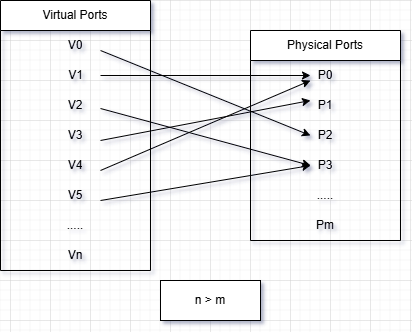
\includegraphics[width=0.4\textwidth]{images/virtual_ports_diagram.png}
        \caption{Mapping of virtual ports to physical pins. Virtual ports v1 and v4 overlap on 
        Physical port p0, while Virtual ports v2 and v5 overlap on Physical port p1.}
      \end{figure}
\end{itemize}

\subsubsection{Physical Pin Configured as Input}
When the physical pin is configured as an input, the virtual port should reflect the data from the physical pin.

\begin{itemize}[noitemsep]
    \item \textbf{Data Flow}: The virtual port reads the value of the physical pin.
    \begin{itemize}[noitemsep]
        \item Any read from the virtual port reflects the current value of the physical pin.
        \item The virtual port is implicitly in input mode.
    \end{itemize}
    \item \textbf{Enable Behavior}: Reading from the virtual port behaves as if reading directly from the physical pin.
    \begin{itemize}[noitemsep]
        \item Virtual port input is enabled when the physical pin input is enabled.
    \end{itemize}
\end{itemize}

\textbf{Example}:
\begin{itemize}[noitemsep]
    \item Physical pin $p$ is set as input.
    \item Virtual port $v$ is mapped to pin $p$.
    \item Reading from virtual port $v$ returns the current value of physical pin $p$ (either $0$ or $1$).
\end{itemize}

\subsubsection{Physical Pin Reconfiguration (Dynamic Behavior)}
If the direction of the physical pin changes dynamically during runtime, the virtual port should reflect this change.

\begin{itemize}[noitemsep]
    \item When a physical pin changes from \textbf{input to output}, the virtual port should switch from \textbf{read-only} to \textbf{write-enabled}.
    \item When a physical pin changes from \textbf{output to input}, the virtual port should switch from \textbf{write-enabled} to \textbf{read-only}.
    \item The virtual port should respect any changes to the physical pin's enable signal (e.g., when a pin is disabled or tri-stated).
\end{itemize}

\subsubsection{Summary of Correspondence}
The following table summarizes the behavior of virtual ports when mapped to physical pins.
\begin{table}[ht]
    \centering
    \resizebox{\textwidth}{!}{%
    \begin{tabular}{|c|c|c|c|}
        \hline
        \textbf{Physical Pin Mode} & \textbf{Virtual Port Behavior} & \textbf{Direction} & \textbf{Enable Behavior} \\ \hline
        \textbf{Output}            & Writes to virtual port propagate to physical pin & Implicit Output & Enabled if physical pin output is enabled \\ \hline
        \textbf{Input}             & Reads from virtual port reflect the physical pin value & Implicit Input  & Enabled if physical pin input is enabled  \\ \hline
    \end{tabular}%
    }
    \caption{Virtual Port Behavior Correspondence with Physical Pins}
\end{table}

\subsubsection{Additional Considerations}

\begin{itemize}[noitemsep]
    \item \textbf{Virtual-to-Physical Map}: Ensure that the \texttt{virtualToPhysicalMap} correctly identifies which physical pin a virtual port is mapped to and maintains this mapping throughout the operation.
    \item \textbf{Enable Flag}: The virtual port enable flag should be checked to ensure that virtual ports are supported. If not enabled, virtual ports should not interact with physical pins.
\end{itemize}

By maintaining consistent mapping and handling between virtual and physical ports, you ensure that virtual ports act as an abstraction layer, extending Gpio functionality without altering the behavior of the physical pins.
